% Options for packages loaded elsewhere
\PassOptionsToPackage{unicode}{hyperref}
\PassOptionsToPackage{hyphens}{url}
%
\documentclass[
]{article}
\usepackage{amsmath,amssymb}
\usepackage{iftex}
\ifPDFTeX
  \usepackage[T1]{fontenc}
  \usepackage[utf8]{inputenc}
  \usepackage{textcomp} % provide euro and other symbols
\else % if luatex or xetex
  \usepackage{unicode-math} % this also loads fontspec
  \defaultfontfeatures{Scale=MatchLowercase}
  \defaultfontfeatures[\rmfamily]{Ligatures=TeX,Scale=1}
\fi
\usepackage{lmodern}
\ifPDFTeX\else
  % xetex/luatex font selection
\fi
% Use upquote if available, for straight quotes in verbatim environments
\IfFileExists{upquote.sty}{\usepackage{upquote}}{}
\IfFileExists{microtype.sty}{% use microtype if available
  \usepackage[]{microtype}
  \UseMicrotypeSet[protrusion]{basicmath} % disable protrusion for tt fonts
}{}
\makeatletter
\@ifundefined{KOMAClassName}{% if non-KOMA class
  \IfFileExists{parskip.sty}{%
    \usepackage{parskip}
  }{% else
    \setlength{\parindent}{0pt}
    \setlength{\parskip}{6pt plus 2pt minus 1pt}}
}{% if KOMA class
  \KOMAoptions{parskip=half}}
\makeatother
\usepackage{xcolor}
\usepackage[margin=1in]{geometry}
\usepackage{graphicx}
\makeatletter
\def\maxwidth{\ifdim\Gin@nat@width>\linewidth\linewidth\else\Gin@nat@width\fi}
\def\maxheight{\ifdim\Gin@nat@height>\textheight\textheight\else\Gin@nat@height\fi}
\makeatother
% Scale images if necessary, so that they will not overflow the page
% margins by default, and it is still possible to overwrite the defaults
% using explicit options in \includegraphics[width, height, ...]{}
\setkeys{Gin}{width=\maxwidth,height=\maxheight,keepaspectratio}
% Set default figure placement to htbp
\makeatletter
\def\fps@figure{htbp}
\makeatother
\setlength{\emergencystretch}{3em} % prevent overfull lines
\providecommand{\tightlist}{%
  \setlength{\itemsep}{0pt}\setlength{\parskip}{0pt}}
\setcounter{secnumdepth}{-\maxdimen} % remove section numbering
\usepackage{amsmath}
\ifLuaTeX
  \usepackage{selnolig}  % disable illegal ligatures
\fi
\IfFileExists{bookmark.sty}{\usepackage{bookmark}}{\usepackage{hyperref}}
\IfFileExists{xurl.sty}{\usepackage{xurl}}{} % add URL line breaks if available
\urlstyle{same}
\hypersetup{
  pdftitle={Urbanization and Public Transportation of Los Angeles},
  pdfauthor={Kainoa Kanter, Julian Jacobson, Aidan Allen},
  hidelinks,
  pdfcreator={LaTeX via pandoc}}

\title{Urbanization and Public Transportation of Los Angeles}
\author{Kainoa Kanter, Julian Jacobson, Aidan Allen}
\date{November 21, 2023}

\begin{document}
\maketitle
\begin{abstract}
This paper will examine how Los Angeles's demand for public
transportation has been affected the last few years, utilizing
derivatives to determine the rate of change in public transportation
usage and studying the elasticity of demand for transportation options
based on pricing, availability, convenience, and modes.
\end{abstract}

\hypertarget{introduction}{%
\section{Introduction}\label{introduction}}

Los Angeles -- the sprawling metropolis that we call home -- has become
synonymous with both opportunity and urban challenges and has
experienced rapid growth in recent decades. This growth has significant
implications for various sectors, particularly the public transportation
system. As one of the most car-dependent cities in the United States,
Los Angeles faces unique challenges in scaling its public transportation
network to meet increasing demand. Understanding the dynamics of public
transportation usage and the factors influencing ridership is critical
for planning and policy development.

The aim of this study is to examine how the rapid growth of Los Angeles
affects the demand for public transportation. The investigation includes
a quantitative assessment utilizing derivatives to determine the rate of
change in public transportation usage. Additionally, the study examines
the elasticity of demand for transportation options in Los Angeles based
on pricing, availability, convenience, and modes. This analysis offers
insights into the responsiveness of ridership to changes in these
factors, informing strategies to enhance the public transportation
system.

\hypertarget{methodology}{%
\subsection{Methodology}\label{methodology}}

\hypertarget{data-collection}{%
\subsubsection{Data Collection}\label{data-collection}}

The analysis is based on comprehensive datasets including average
weekend and weekday ridership from 2019 to 2023, as well as a range of
urban metrics such as crime rates, accident statistics, and city
maintenance records. Yearly transportation budget figures also
contribute to understanding the financial aspects influencing public
transportation operations.

The methodological approach consists of two primary quantitative
analyses:

\hypertarget{rate-of-change-analysis}{%
\paragraph{Rate of Change Analysis:}\label{rate-of-change-analysis}}

\begin{itemize}
\tightlist
\item
  Utilize time-series data to calculate the first derivative of
  ridership numbers, yielding the rate of change over the years. This
  derivative analysis will be conducted separately for bus and rail
  services, offering a granular view of usage trends.
\item
  Data transformation into a suitable format for analysis using the
  tidyverse collection of R packages.
\item
  Visualization of trends through line plots, elucidating patterns and
  growth trajectories.
\end{itemize}

\hypertarget{elasticity-of-demand-analysis}{%
\paragraph{Elasticity of Demand
Analysis:}\label{elasticity-of-demand-analysis}}

\begin{itemize}
\item
  Analyze the responsiveness of public transportation demand to changes
  in price (fare changes), availability (service hours, frequency),
  convenience (route changes, wait times), and modes (bus vs.~rail).
\item
  Employ econometric modeling to estimate the price elasticity of
  demand, cross-elasticity, and income elasticity, using regression
  analysis where ridership
\end{itemize}

\hypertarget{visualization}{%
\paragraph{Visualization}\label{visualization}}

\begin{itemize}
\tightlist
\item
  Data visualization was implemented using the \texttt{ggplot2} package
  in R
\item
  Line plots were created to illustrate the trends in public
  transportation ridership over time, broken down by transportation type
  (bus and rail)
\item
  Adjustments were made to display actual numbers instead of scientific
  notation for clarity
\end{itemize}

\newpage

\hypertarget{exploratory-data-analysis}{%
\section{Exploratory Data Analysis}\label{exploratory-data-analysis}}

\begin{figure}
\centering
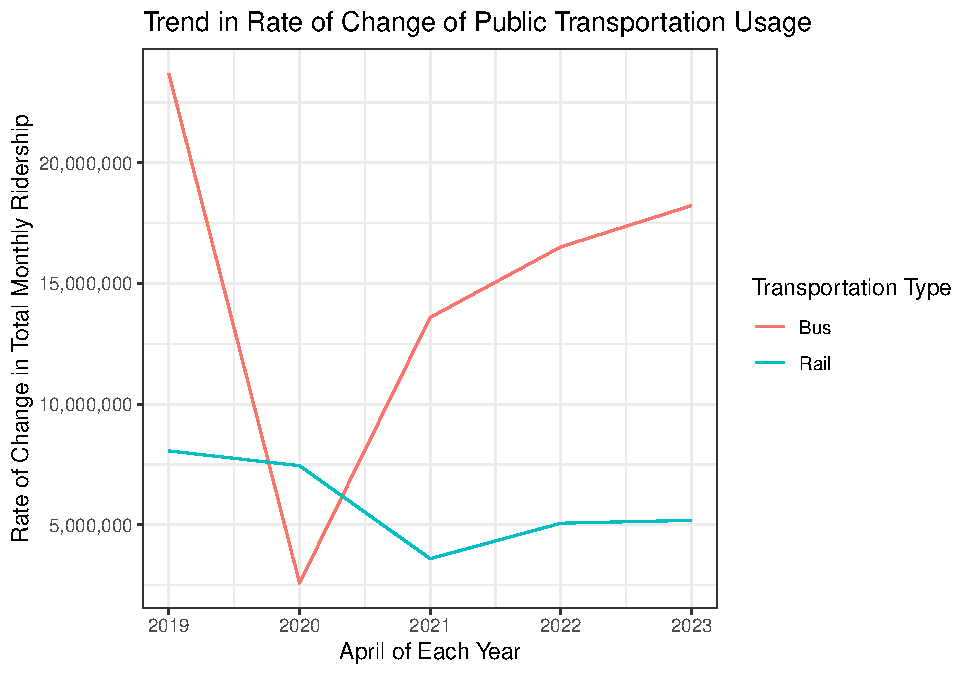
\includegraphics{Paper_files/figure-latex/rate-of-change-plot-1.pdf}
\caption{Line plot of rate of change in public transportation ridership
over time}
\end{figure}

\newpage

\hypertarget{derivative-analysis}{%
\section{Derivative Analysis}\label{derivative-analysis}}

The rate of change in public transportation usage offers valuable
insights into trends and can help forecast future demand. By
differentiating the ridership data with respect to time, we can obtain
the instantaneous rate of change, which is expressed mathematically as:

\[
R'(t) = \frac{dR}{dt}
\]

where \(R(t)\) represents the ridership at time \(t\). This derivative
analysis provides the velocity of ridership change, indicating whether
usage is increasing or decreasing over time.

\begin{table}[!htbp] \centering 
  \caption{Linear Regression Results} 
  \label{} 
\begin{tabular}{@{\extracolsep{5pt}}lcc} 
\\[-1.8ex]\hline 
\hline \\[-1.8ex] 
 & \multicolumn{2}{c}{\textit{Dependent variable:}} \\ 
\cline{2-3} 
\\[-1.8ex] & BusRateOfChange & RailRateOfChange \\ 
\\[-1.8ex] & (1) & (2)\\ 
\hline \\[-1.8ex] 
\hline \\[-1.8ex] 
Observations & 4 & 4 \\ 
R$^{2}$ & 0.319 & 0.184 \\ 
Adjusted R$^{2}$ & $-$0.021 & $-$0.223 \\ 
Residual Std. Error (df = 2) & 13,934,596.000 & 2,498,636.000 \\ 
F Statistic (df = 1; 2) & 0.938 & 0.452 \\ 
\hline 
\hline \\[-1.8ex] 
\textit{Note:}  & \multicolumn{2}{r}{$^{*}$p$<$0.1; $^{**}$p$<$0.05; $^{***}$p$<$0.01} \\ 
\end{tabular} 
\end{table}

\begin{table}[!htbp] \centering 
  \caption{Polynomial Regression Results} 
  \label{} 
\begin{tabular}{@{\extracolsep{5pt}}lcc} 
\\[-1.8ex]\hline 
\hline \\[-1.8ex] 
 & \multicolumn{2}{c}{\textit{Dependent variable:}} \\ 
\cline{2-3} 
\\[-1.8ex] & BusRateOfChange & RailRateOfChange \\ 
\\[-1.8ex] & (1) & (2)\\ 
\hline \\[-1.8ex] 
\hline \\[-1.8ex] 
Observations & 4 & 4 \\ 
R$^{2}$ & 0.806 & 0.243 \\ 
Adjusted R$^{2}$ & 0.418 & $-$1.272 \\ 
Residual Std. Error (df = 1) & 10,522,144.000 & 3,405,367.000 \\ 
F Statistic (df = 2; 1) & 2.076 & 0.160 \\ 
\hline 
\hline \\[-1.8ex] 
\textit{Note:}  & \multicolumn{2}{r}{$^{*}$p$<$0.1; $^{**}$p$<$0.05; $^{***}$p$<$0.01} \\ 
\end{tabular} 
\end{table}

\[ \text{Total\ Monthly\ Bus} = -16456298.50 + 6036028.40 \cdot (Year - 2019) \]\[ \text{Total\ Monthly\ Rail} = -2597795.50 + 751531.80 \cdot (Year - 2019) \]\[ \text{Total\ Monthly\ Bus} = -58111913.49 + 33688766315.52 \cdot (Year - 2019) + -8331123.00 \cdot (Year - 2019)^2 \]\[ \text{Total\ Monthly\ Rail} = -239513.00 + -1906155697.79 \cdot (Year - 2019) + 471656.50 \cdot (Year - 2019)^2 \]

\begin{figure}
\centering
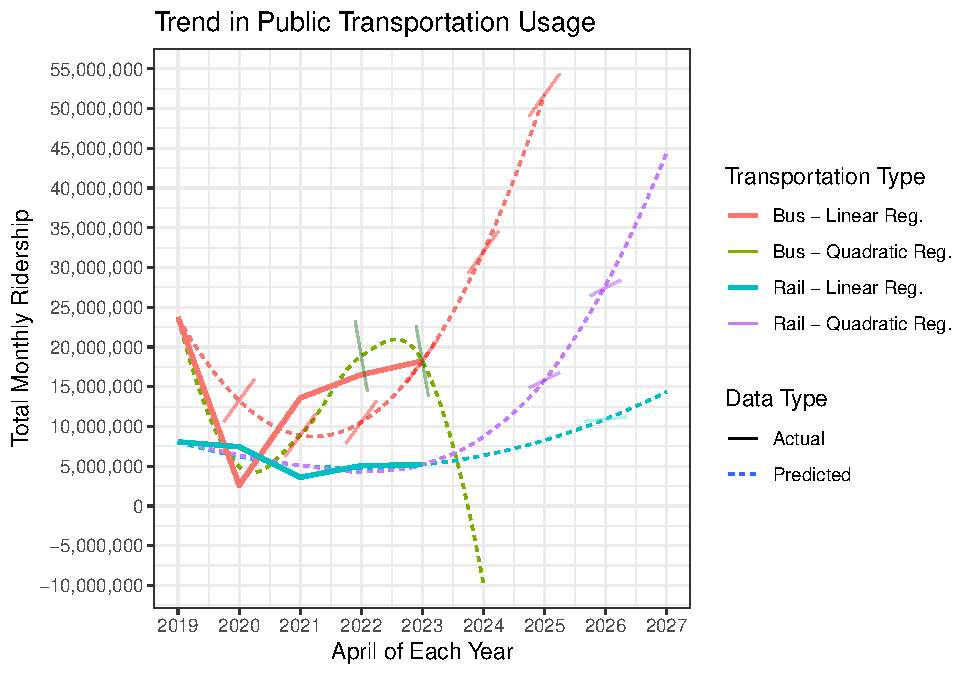
\includegraphics{Paper_files/figure-latex/plot-trend-usage-1.pdf}
\caption{Line plot of public transportation ridership over time with
regression lines}
\end{figure}

\newpage

\hypertarget{sources}{%
\section{Sources:}\label{sources}}

\begin{itemize}
\tightlist
\item
  Transit ridership data: Los Angeles Metro ``L.A. METRO TRANSIT
  RIDERSHIP UP 10 PERCENT, SETS POST-PANDEMIC RECORD'', Patrick Chandler
\end{itemize}

\end{document}
